\chapter{Subject of the thesis}
\label{chapter:3_subject}

\section{Test application}
% TODO: describe what you wrote

\section{Implemented shadow rendering techniques}
Below, all the shadow rendering techniques that have been implemented during work on this thesis are described, along with explanations of their algorithms.

\subsection{Planar shadows implementation}
\label{section:planar_shadows_impl}

Planar shadows, as described in section \ref{section:planar_shadows}, are a very simple technique to achieve hard shadows, introduced by Blinn \cite{bib:article:blinn_shadows}. The idea for the algorithm stems from the geometric understanding of how a shadow is formed. The shape of a shadow is basically the shadow caster projected onto the surface of a shadow receiver along rays from a light source, as shown in Fig. \ref{fig:projection_shadow}. 

\begin{figure}[h]
	\centering
	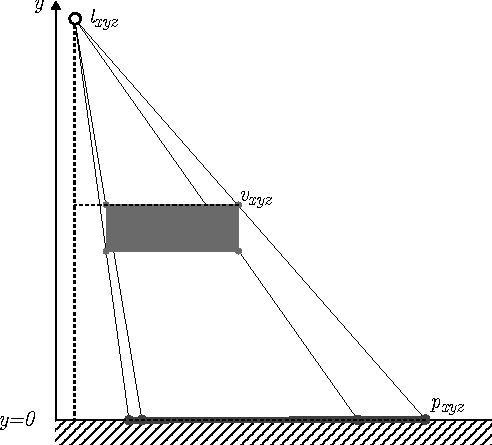
\includegraphics[width=0.5\textwidth]{./graf/projection_shadow.pdf}
	\caption{Vertices of a shadow caster projected onto \(y=0\) plane create a planar shadow. Dashed lines visualize the similar triangles.}
	\label{fig:projection_shadow}
\end{figure}

Using this geometric understanding and similar triangles, marked in Fig. \ref{fig:projection_shadow} in dashed lines, the following equations and a projection matrix can be derived. Assuming \(l\) to be the position of a light source, \(v\) to be the position of a vertex of the shadow caster and \(p\) the position of the projected shadow vertex, a projection onto the \(y=0\) plane is described by:

\begin{align}
	\frac{p_x - l_x}{v_x - l_x} = \frac{l_y}{l_y - v_y} \Longleftrightarrow p_x = \frac{l_yv_x - l_xv_y}{l_y - v_y}
\end{align}

The \(z\) component is derived in analogous way:

\begin{align}
	\frac{p_z - l_z}{v_z - l_z} = \frac{l_y}{l_y - v_y} \Longleftrightarrow p_z = \frac{l_yv_z - l_zv_y}{l_y - v_y}
\end{align}

The \(y\) component will be \(y=0\) since the projection happens onto the \(xz\) plane. From that the projection matrix can be constructed:

\begin{align}
	\mathbf{M} = 
	\begin{pmatrix}
		l_y & -l_x & 0 & 0\\
		0 & 0 & 0 & 0\\
		0 & -l_z & l_y & 0\\
		0 & -1 & 0 & l_y
	\end{pmatrix}
\end{align}

The \(l_y - v_y\) factor in the denominator is obtained by utilizing the property of homogenous coordinates, where all components of a vector \(\mathbf{v} = \begin{bmatrix}x & y & z & w\end{bmatrix}^T\) get divided by the \(w\) component, which gives \(\mathbf{v} = \begin{bmatrix}x/w & y/w & z/w & 1\end{bmatrix}^T\).

This matrix can be generalized to project points onto any plane, but this was not implemented.

In the implementation the matrix is created in the vertex shader based on the position of the light source. The vertices of the caster, after being transformed into world space, are multiplied by it, projecting them onto the \(y=0\) plane. Then they are transformed with the view and perspective projection matrices as usual. The resulting mesh is rendered in black, with a pixel shader that just returns the black color. Special care should be taken when rendering the shadow mesh, since it perfectly overlaps the ground plane at \(y=0\). To avoid z-fighting this mesh needs to be rendered after the receiver and before the caster, with z depth testing turned off in the rendering pipeline, or, as is the case in the implementation, a negative depth offset needs to be added to the mesh to bring it above the ground plane.

% TODO: add z-fighting image, add shadow beyond receiver image.

Multiple issues arise with this technique. The receiver must be a flat plane, objects cannot shadow themselves, casters and receivers need separate treatment. Additionally, care needs to be taken to only render the shadow meshes on top of the geometry of a receiver. Since the shadow is a separate mesh, it could be cast beyond the actual surface of the receiver, creating an impossible shadow in the air. There is another possibility here for an impossible shadow. If the light source is between the caster and receiver, an anti-shadow will be cast as shown in Fig \ref{fig:projection_anti_shadow}. This creates another special case that needs to be checked for by the application. Soft shadows are also difficult and costly to achieve, created by projecting the caster geometry multiple times using different discrete locations sampled over the area of the light source. The shadow meshes can then be blended, producing a darker color where more shadows are present. This gives very accurate results with a high number of samples, but is not a viable option for real-time rendering. All these problems make this technique virtually unused in modern rendering engines.

\begin{figure}
	\centering
	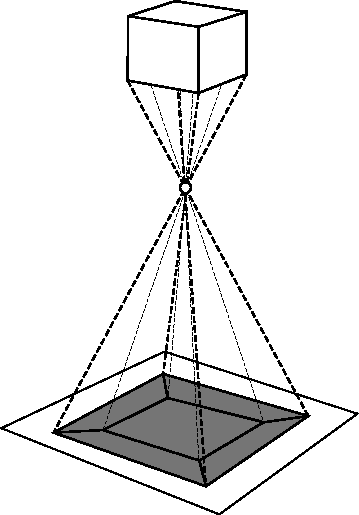
\includegraphics[width=0.3\textwidth]{./graf/projection_anti_shadow.pdf}
	\caption{The shadow caster projected through a light source, creating an anti-shadow.}
	\label{fig:projection_anti_shadow}
\end{figure}

% TODO: add some notes on performance.

\begin{itemize}
\item solution to the problem proposed by the author of the thesis
\item theoretical analysis of proposed solutions
\item rationale of applied methods, algorithms, and tools
\end{itemize}

Here I should describe my reasoning for the testing, reasoning for
selecting the techniques that I do select, my program for testing.

\section{[Section title]}

\section{[Subsection title]}

Each figure in the document should be referred to at least once (fig. \ref{fig:2}).

\begin{figure}
\centering
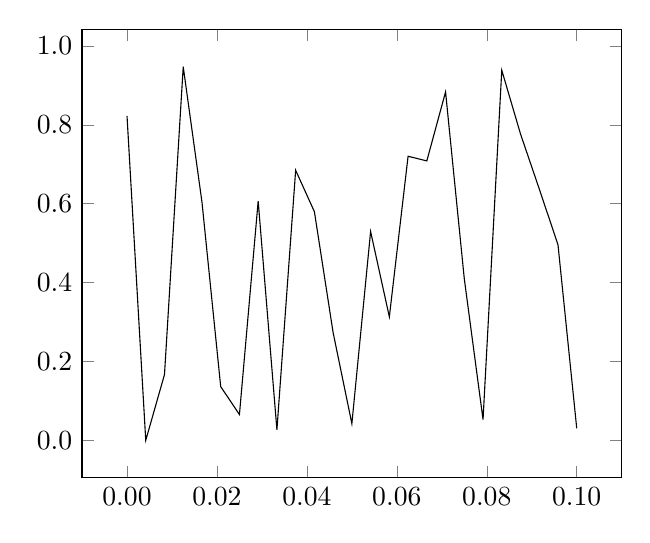
\begin{tikzpicture}
\begin{axis}[
    y tick label style={
        /pgf/number format/.cd,
            fixed,   % po zakomentowaniu os rzednych jest indeksowana wykladniczo
            fixed zerofill, % 1.0 zamiast 1
            precision=1,
        /tikz/.cd
    },
    x tick label style={
        /pgf/number format/.cd,
            fixed,
            fixed zerofill,
            precision=2,
        /tikz/.cd
    }
]
\addplot [domain=0.0:0.1] {rnd};
\end{axis} 
\end{tikzpicture}
\caption{Figure caption.} % Figure caption is BELOW the figure!
\label{fig:2}
\end{figure}


%%%%%%%%%%%%%%%%%%%%%
% FIGURE FROM FILE
%
%\begin{figure}
%\centering
%
\includegraphics[width=0.5\textwidth]{./graf/politechnika_sl_logo_bw_pion_en.pdf}
%\caption{Caption of a figure is always below the figure.}
%\label{fig:label}
%\end{figure}
%Fig. \ref{fig:label} presents …
%%%%%%%%%%%%%%%%%%%%%
%
%%%%%%%%%%%%%%%%%%%%
%% SUBFIGURES
%
%\begin{figure}
%\centering
%\begin{subfigure}{0.4\textwidth}
%    
\includegraphics[width=\textwidth]{./graf/politechnika_sl_logo_bw_pion_en.pdf}
%    \caption{Upper left figure.}
%    \label{fig:upper-left}
%\end{subfigure}
%\hfill
%\begin{subfigure}{0.4\textwidth}
%    
\includegraphics[width=\textwidth]{./graf/politechnika_sl_logo_bw_pion_en.pdf}
%    \caption{Upper right figure.}
%    \label{fig:upper-right}
%\end{subfigure}
%
%\begin{subfigure}{0.4\textwidth}
%    
\includegraphics[width=\textwidth]{./graf/politechnika_sl_logo_bw_pion_en.pdf}
%    \caption{Lower left figure.}
%    \label{fig:lower-left}
%\end{subfigure}
%\hfill
%\begin{subfigure}{0.4\textwidth}
%    
\includegraphics[width=\textwidth]{./graf/politechnika_sl_logo_bw_pion_en.pdf}
%    \caption{Lower right figure.}
%    \label{fig:lower-right}
%\end{subfigure}
%        
%\caption{Common caption for all subfigures.}
%\label{fig:subfigures}
%\end{figure}
%Fig. \ref{fig:subfigures} presents very important information, eg. Fig. \ref{fig:upper-right} is an upper right subfigure.
%%%%%%%%%%%%%%%%%%%%%


Each table in the document should be referred to at least once (Tab. \ref{tab:results}).

\begin{table}
\centering
\caption{A caption of a table is ABOVE it.}
\label{tab:results}
\begin{tabular}{rrrrrrrr}
\toprule
	         &                                     \multicolumn{7}{c}{method}                                      \\
	         \cmidrule{2-8}
	         &         &         &        \multicolumn{3}{c}{alg. 3}        & \multicolumn{2}{c}{alg. 4, $\gamma = 2$} \\
	         \cmidrule(r){4-6}\cmidrule(r){7-8}
	$\zeta$ &     alg. 1 &   alg. 2 & $\alpha= 1.5$ & $\alpha= 2$ & $\alpha= 3$ &   $\beta = 0.1$  &   $\beta = -0.1$ \\
\midrule
	       0 &  8.3250 & 1.45305 &       7.5791 &    14.8517 &    20.0028 & 1.16396 &                       1.1365 \\
	       5 &  0.6111 & 2.27126 &       6.9952 &    13.8560 &    18.6064 & 1.18659 &                       1.1630 \\
	      10 & 11.6126 & 2.69218 &       6.2520 &    12.5202 &    16.8278 & 1.23180 &                       1.2045 \\
	      15 &  0.5665 & 2.95046 &       5.7753 &    11.4588 &    15.4837 & 1.25131 &                       1.2614 \\
	      20 & 15.8728 & 3.07225 &       5.3071 &    10.3935 &    13.8738 & 1.25307 &                       1.2217 \\
	      25 &  0.9791 & 3.19034 &       5.4575 &     9.9533 &    13.0721 & 1.27104 &                       1.2640 \\
	      30 &  2.0228 & 3.27474 &       5.7461 &     9.7164 &    12.2637 & 1.33404 &                       1.3209 \\
	      35 & 13.4210 & 3.36086 &       6.6735 &    10.0442 &    12.0270 & 1.35385 &                       1.3059 \\
	      40 & 13.2226 & 3.36420 &       7.7248 &    10.4495 &    12.0379 & 1.34919 &                       1.2768 \\
	      45 & 12.8445 & 3.47436 &       8.5539 &    10.8552 &    12.2773 & 1.42303 &                       1.4362 \\
	      50 & 12.9245 & 3.58228 &       9.2702 &    11.2183 &    12.3990 & 1.40922 &                       1.3724 \\
\bottomrule
\end{tabular}
\end{table}  


\begin{figure}
\centering
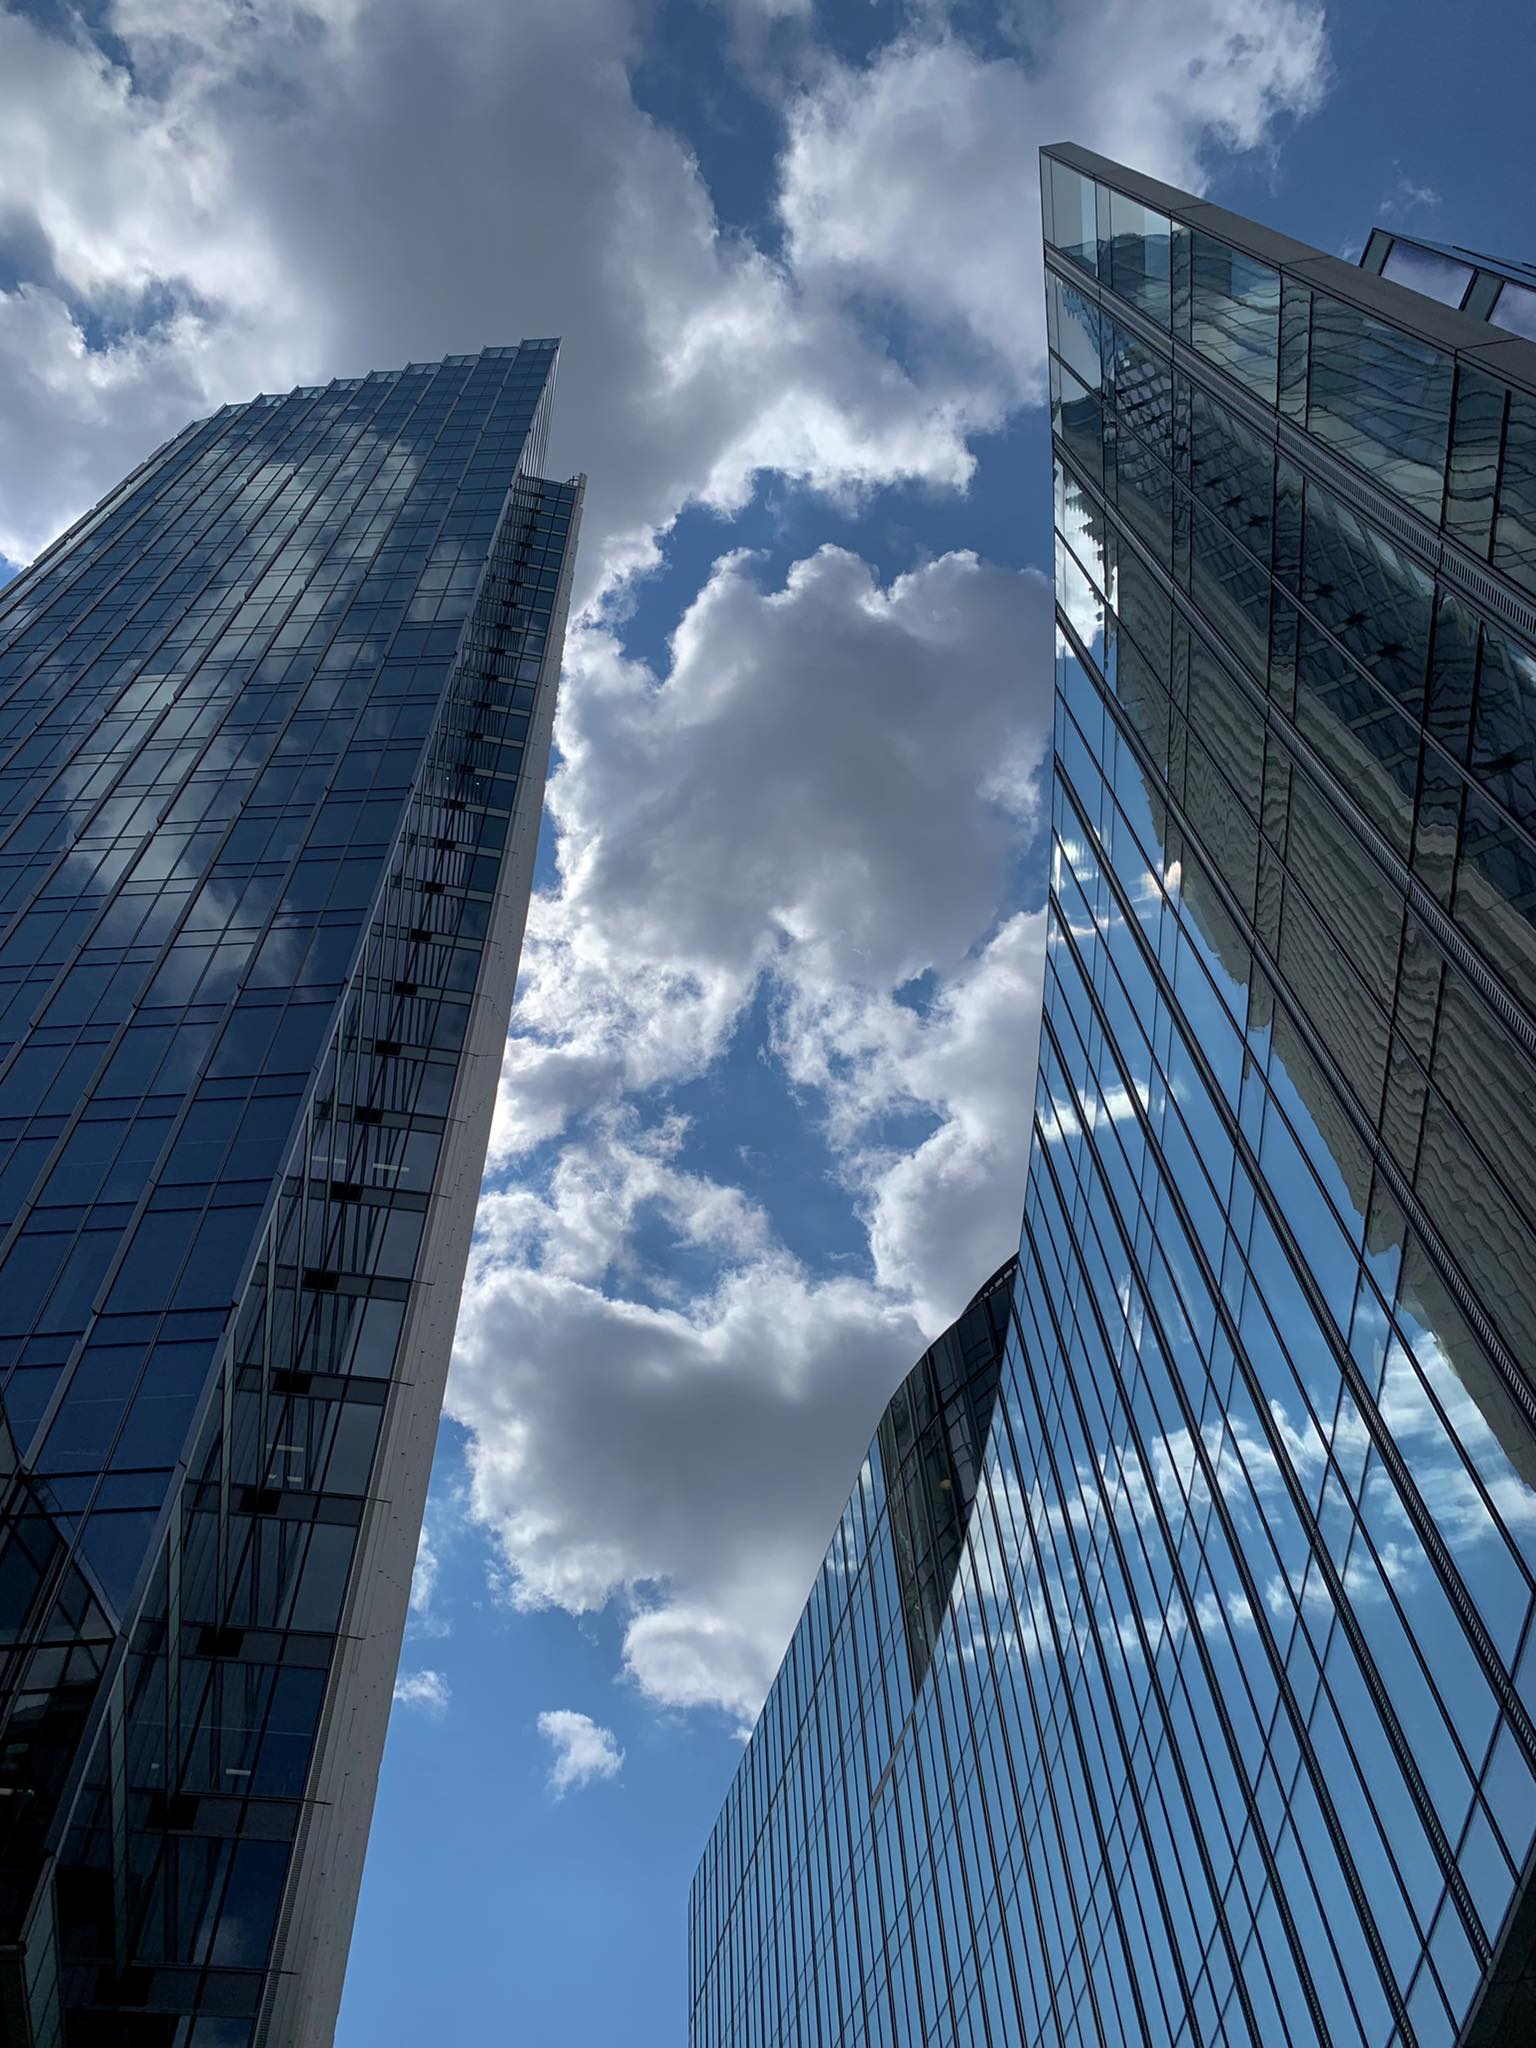
\includegraphics[width=0.5\textwidth]{./graf/test_image.jpg}
\caption{Caption of a figure is always below the figure akakak.}
\label{fig:duped_image4}
\end{figure}

some citation of the above \ref{fig:duped_image4}
